
\begin{activite}[Du côté des triangles \ldots]

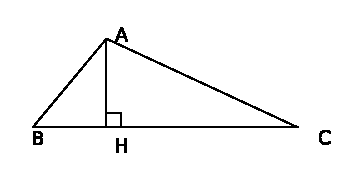
\includegraphics[width=4.8cm]{triangleABCH}

\begin{enumerate}
\item Donne d'autres écritures de l'angle $\widehat{ABC}$ \dotfill

\item Quel angle du triangle $AHC$ possède la plus petite mesure ?  \dotfill

\item Dans le triangle $ABC$, quel est le côté opposé au sommet $B$ ?  \dotfill

\item Dans le triangle $AHC$, quel est le sommet opposé au côté $[HC]$ ?  \dotfill

\item Quel est l'angle droit du triangle $HAB$ ?  \dotfill

\item Quels sont les noms des trois angles du triangle $ACH$ ?  \dotfill

\item Dans cette figure, quels sont les angles aigus, droits et obtus ?  \dotfill

 \dotfill

 \dotfill
\end{enumerate}

\end{activite}

%%%%%%%%%%%%%%%%%%%%%%%%%%%%%%%%%%%%%%%%%%%%%%%%%%%%%%%%%%%%%%%

\begin{activite}[Du côté des triangles particuliers \ldots]

Romuald doit construire un triangle $IJK$ rectangle en $I$, Isabelle un triangle $EFG$ isocèle en $F$ et Eddy un triangle équilatéral $QRS$.

\begin{enumerate}

\item Trace trois figures à main levée pour représenter ces triangles et code-les.

\vspace{4cm}
\item Dans le triangle $IJK$, quel nom donne-t-on au côté $[JK]$ ? \dotfill

\item Dans le triangle $EFG$, quelle est la base ? Quel est le sommet principal ? Que peut-on dire des côtés $[EF]$ et $[GF]$ ? Que peut-on dire des angles $\widehat{FEG}$ et $\widehat{FGE}$ ?  \dotfill

 \dotfill

\item Que peut-on dire des côtés du triangle $QRS$ ? Et de ses angles ?  \dotfill

\item En observant le codage, indique la nature des triangles ci-dessous :


\includegraphics[width=2.3cm]{triangle_rose} \hfill 
\includegraphics[width=1.8cm]{triangle_vert} \hfill 
\includegraphics[width=2.1cm]{triangle_bleu} \hfill 
\includegraphics[width=1.9cm]{triangle_orange}

\end{enumerate}

\end{activite}

%%%%%%%%%%%%%%%%%%%%%%%%%%%%%%%%%%%%%%%%%%%%%%%%%%%%%%%%%%%%%%%

\begin{activite}[Somme des angles d'un triangle]

\begin{enumerate}
\item Trace deux triangles quelconques de formes différentes et mesure leurs angles à l'aide d'un rapporteur.

\item Trace un triangle particulier (isocèle, rectangle ou équilatéral) puis mesure ses angles à l'aide d'un rapporteur.

\item Pour chacun des trois triangles tracés, additionne les mesures de ses trois angles. Que remarques-tu ?

\item Essaie de tracer un triangle dont la somme des angles vaut $220^\circ$. Que remarques-tu ?
\end{enumerate}

\end{activite}

%%%%%%%%%%%%%%%%%%%%%%%%%%%%%%%%%%%%%%%%%%%%%%%%%%%%%%%%%%%%%%%

\begin{activite}[Hasardons-nous à construire un triangle]

\begin{enumerate}
\item Choisis trois nombres compris entre 2 et 15. Note-les sur ton cahier. Effectue un croquis d'un triangle dont les trois nombres choisis sont les mesures de ses côtés (en cm).

\item Essaie de le construire en vraie grandeur.

\item Penses-tu qu'il soit possible de construire le triangle représenté par le croquis ci-dessous ? Justifie.

\begin{center} 
\includegraphics[width=2.9cm]{triangleLMK} \end{center}
\end{enumerate}

\end{activite}

%%%%%%%%%%%%%%%%%%%%%%%%%%%%%%%%%%%%%%%%%%%%%%%%%%%%%%%%%%%%%%%

\begin{activite}[Constructible ou non ?]
Un professeur demande à ses élèves de construire le triangle $ABC$ donné par le croquis ci-contre. Voici les réponses de quatre élèves : \\[1em]
\begin{minipage}[t]{0.46\textwidth}
\begin{itemize}
 \item Kim dit que le triangle $ABC$ est constructible puisque la figure est tracée ;
 \item Jordan dit que, comme $4 < 6 + 11$,  le triangle $ABC$ est constructible ;
 \item Mickaël dit qu'il est d'accord avec Jordan car en plus $6 < 11 + 4$ ;
 \item Imad dit que l'inégalité $11 < 6 + 4$ est fausse et que le triangle $ABC$ n'est donc pas constructible.
 \end{itemize}
\end{minipage} \hfill%
\begin{minipage}[t]{0.36\textwidth}
\hfill \\
\begin{center} 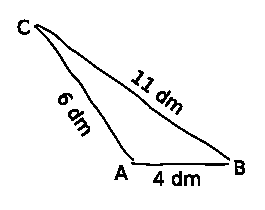
\includegraphics[width=3.8cm]{triangleCAB} \end{center}
\end{minipage} \\

\begin{enumerate}
\item Que penses-tu de chacune des réponses ? Qui a raison ?

\item Au total, combien d'inégalités ont été proposées par ces élèves ? Pour savoir si le triangle $ABC$ est constructible, faut-il vérifier toutes ces inégalités ?
   
\item Effectue un croquis d'un triangle \underline{non} constructible ayant des côtés mesurant 7,5 m, 12 m et une troisième valeur de ton choix, plus grande que les deux autres.
         
\item Effectue un croquis d'un triangle \underline{non} constructible ayant des côtés mesurant 6,5 km, 10 km et une troisième valeur de ton choix, plus petite que les deux autres.
\end{enumerate}

\end{activite}


%%%%%%%%%%%%%%%%%%%%%%%%%%%%%%%%%%%%%%%%%%%%%%%%%%%%%%%%%%%%%%%

\begin{activite}[Une figure à main levée \ldots à l'œil ouvert]

Voici quatre croquis d'un triangle $AKL$ tel que $AK = 5$ cm, $\widehat{LAK} = 47^\circ$ et $\widehat{LKA} = 96^\circ$ :
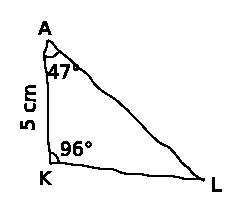
\includegraphics[width=3.3cm]{triangleAKL_1} \hfill 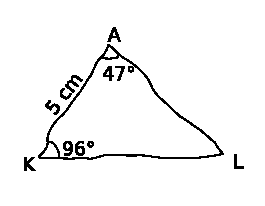
\includegraphics[width=3.4cm]{triangleAKL_2} \hfill 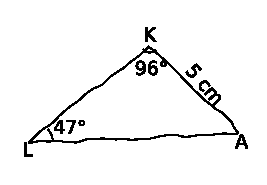
\includegraphics[width=3.8cm]{triangleAKL_3} \hfill 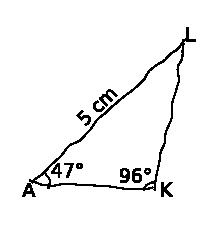
\includegraphics[width=2.7cm]{triangleAKL_4}

\qquad croquis 1 \hfill croquis 2 \hfill croquis 3 \hfill croquis 4 \hfill \\[0.2em]

\begin{enumerate}

\item Quels sont les croquis corrects ?  \dotfill

\item Construis le triangle $AKL$.
\end{enumerate}

\end{activite}


%%%%%%%%%%%%%%%%%%%%%%%%%%%%%%%%%%%%%%%%%%%%%%%%%%%%%%%%%%%%%%%

\begin{activite}[Une figure à main levée \ldots à l'œil ouvert (bis)]

Voici cinq croquis d'un triangle $NPS$ isocèle en $N$ tel que $NS = 4$ cm et $\widehat{SNP} = 75^\circ$ :

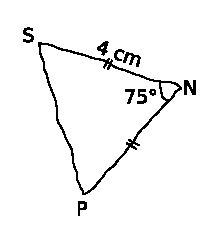
\includegraphics[width=2.6cm]{triangleSNP_1} \hfill 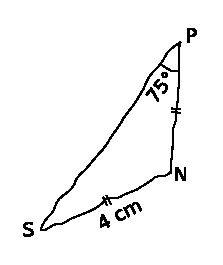
\includegraphics[width=2.4cm]{triangleSNP_2} \hfill 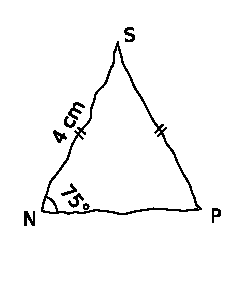
\includegraphics[width=2.9cm]{triangleSNP_3} \hfill 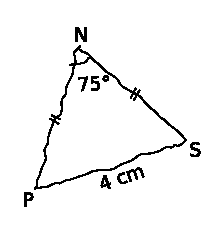
\includegraphics[width=2.7cm]{triangleSNP_4} \hfill 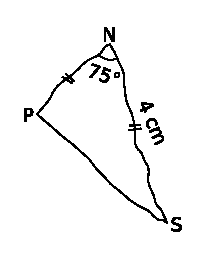
\includegraphics[width=2.5cm]{triangleSNP_5} 

\quad croquis 1 \hfill croquis 2 \hfill croquis 3 \hfill croquis 4 \hfill croquis 5 \\[0.2em]

\begin{enumerate}

\item Quels sont les croquis corrects ? \dotfill

\item En commençant par le segment $[NS]$, construis le triangle $NPS$.
\end{enumerate}

\end{activite}
